\subsection{ZAP Proxy}

Wie in \autoref{ch:sicherheit} erwähnt, müssen beide Versionen von jExam
auf größere Sicherheitslücken gescannt werden. Schwachstellen-Scanner für
Webanwendungen sind automatisierte Tools, die Webanwendungen - normalerweise
von außen - auf Sicherheitslücken wie Cross-Site-Scripting, SQL Injektion,
Command Injektion, Path Traversal und unsichere Serverkonfiguration
untersuchen (vgl. \cite{vulscan}). Diese Kategorie von Tools wird häufig
als Dynamic Application Security Testing (\acs{dast}) Tools bezeichnet.
Es gibt eine große Anzahl kommerzieller und Open-Source-Tools dieser Art,
und alle diese Tools haben ihre eigenen Stärken und Schwächen. Die Analyse
der verschiedenen Tools zum Aufspüren von Schwachstellen wird in dieser
Arbeit nicht behandelt. Es gibt jedoch das OWASP Benchmark-Projekt
(vgl \cite{benchmark}), das die Effektivität aller Arten von Tools zum
Aufspüren von Schwachstellen, einschließlich \asc{dast}, wissenschaftlich
misst. Das Tool zum Scannen von Schwachstellen, das in dieser Arbeit verwendet wird,
ist ZAP Proxy.

\acs{zap} steht für Zed Attack Proxy und bezeichnet eine
Open-Source-Sicherheitssoftware, die in der Programmiersprache Java
geschrieben und 2010 veröffentlicht wurde. Sie wird verwendet, um
Webanwendungen auf Schwachstellen zu scannen. Es wurde als kleines
Projekt vom Open Web Application Security Project (OWASP) gestartet und
ist heute das aktivste Projekt, das von Tausenden von Menschen auf der
ganzen Welt betreut wird. Es ist der am häufigsten verwendete
Webanwendungsscanner (vgl. \cite{zap}). \acs{zap} ist für Linux, Windows und Mac
in 29 Sprachen verfügbar. Zed Attack Proxy wird verwendet, um
Schwachstellen auf beliebigen Webservern zu erkennen. Zu den wichtigsten
Schwachstellen, die von \asc{zap} erkannt werden können, gehören :

\begin{enumerate}
    \item SQL injektion (Injection)
    \item Fehler in der Authentifizierung (Broken Authentication)
    \item Verlust der Vertraulichkeit von Daten (Sensitive data exposure)
    \item Fehler in der Zugriffskontrolle (Broken Access control)
    \item Sicherheitsrelevante Fehlkonfiguration (Security misconfiguration)
    \item Cross Site Scripting (XSS)
    \item Unsichere Deserialisierung (Insecure Deserialization)
    \item Nutzung von Komponenten mit bekannten Schwachstellen (Components with known vulnerabilities)
    \item Fehlende Sicherheitsheader (Missing security headers)
\end{enumerate}

Was Zap zum meistgenutzten Werkzeug für Sicherheitsprüfungen macht,
ist in erster Linie die Tatsache, dass es nicht nur für die Verwendung
durch erfahrene Penetrationstester, sondern auch für Anfänger auf diesem
Gebiet konzipiert wurde. ZAP ist ein kostenloses Open-Source-Tool, das
einfach einzurichten und zu verwenden ist. Da es von einer breiten Community
verwendet wird, gibt es online im ZAP-Blog und in anderen Artikeln eine Menge
Hilfe, die Ihnen bei der Einrichtung und Verwendung des Tools hilft.
ZAP kann in einem Docker-Container ausgeführt werden. Außerdem ist die
Funktionalität skalierbar mit vielen verschiedenen Erweiterungen, die
auf GitHub veröffentlicht wurden.


ZAP ist ein so genannter "Man-in-the-middle-Proxy". Er wird zwischen den
Browser und die Webanwendung geschaltet. Während der Tester durch alle
Funktionen der Website navigiert, erfasst er alle Aktionen. Anschließend
greift er die Website mit bekannten Techniken an, um Sicherheitslücken zu
finden.  ZAP ist ein Werkzeug, das menschliche Intelligenz benötigt,
um richtig eingesetzt zu werden (es ist manuelles Werkzeug).
Penetrationstester verwenden es zunächst, um automatisch nach Schwachstellen
in einer Webanwendung zu scannen. Sobald sie eine Schwachstelle gefunden
haben, die sie ausnutzen können, verwenden sie ZAP, um die Anwendung
anzugreifen. Wie bereits in \autoref{ch:sicherheit} erwähnt, ist die einzige Funktion,
die jExam verwenden wird, der Scanner. Es geht darum, die Anwendung zu
scannen, um größere Sicherheitslücken zu finden.  Wenn die Anwendung solche
Lücken enthält, ist es für die Entwickler unerlässlich, zu handeln und
herauszufinden, wie man sie beheben kann. Auf diese Weise ist es möglich,
ZAP vollautomatisch zu verwenden.


\begin{figure}[H]
    \centering
    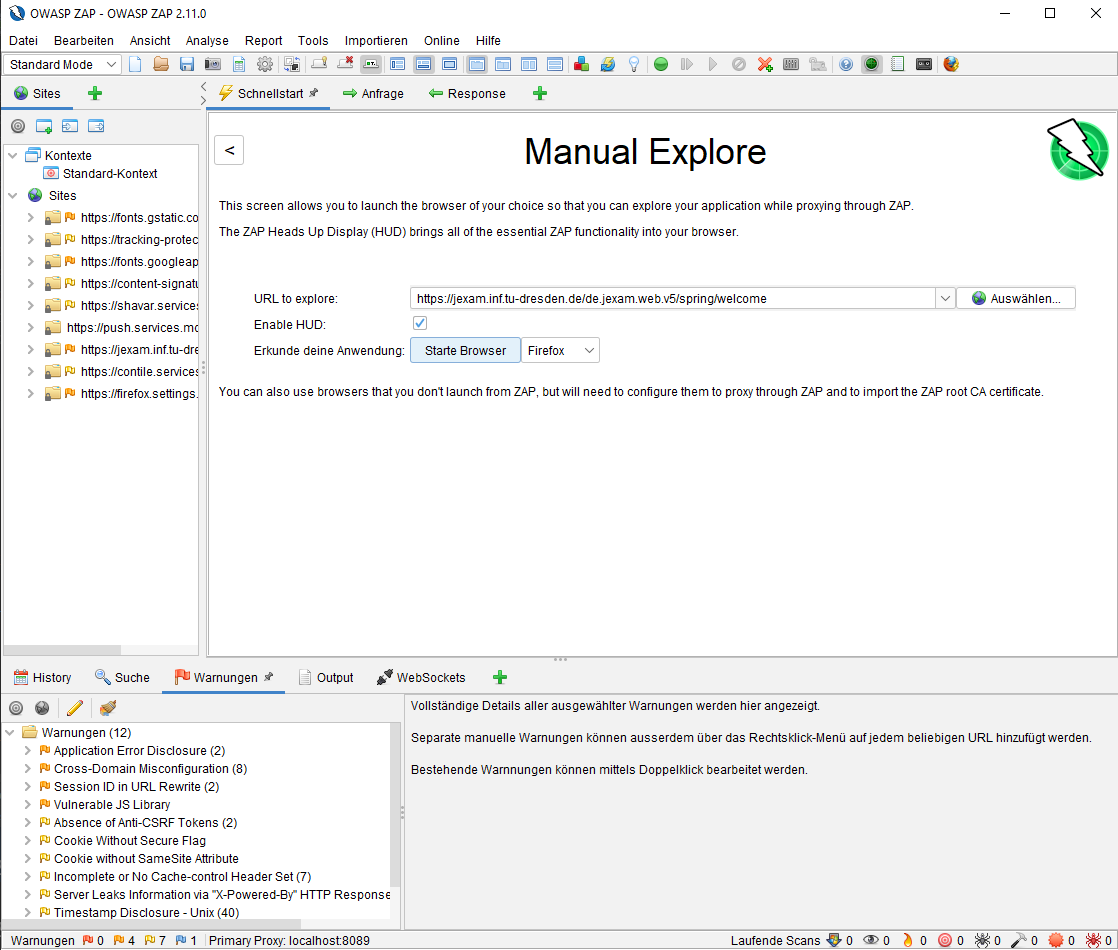
\includegraphics[scale=0.5]{images/zap-interface}
    \caption{Grafische Benutzeroberfläche von Zap} \label{fig:zap-interface}
\end{figure}


